\chapter{Deterministic Execution}
Deterministic execution provides a property that given the same input, a multithreaded program can always generate the same output. Such a system fits perfectly for our replication purpose. Among all the deterministic systems, there is one type called "Weak Deterministic System". Those systems assume the applications are race free, and only guarantee the deterministic interleaving of thread synchronization primitives such as mutex locks and condition variables. Our implementation falls into this category, we implemented a set of system calls to control the application's behaviour. By putting our system calls around the synchronization primitives, we are able to control the interleaving of those code sections.

\section{Logical Time Based Deterministic Scheduling}
Inspired by Kendo\cite{olszewski2009kendo} and Conversion\cite{merrifieldincreasing}, this scheduling policy maintains a logical time for each task inside the namespace. Our system provides three system calls for the applications to control the thread-interleaving:
\begin{itemize}
   \item \_\_det\_start: Upon it is called, only the task holds the minimal logical time can proceed, if several tasks have the same logical time, the one who has the smallest PID number gets the turn. If the current thread is able to proceed, this thread will be marked as "in a deterministic section".
   \item \_\_det\_end: When is called, the system will increase the current thread's logical by 1, and marks it as "out of a deterministic section".
   \item \_\_det\_tick: This system call comes with a parameter of an integer. When it is called, the logical time will be increased by value defined by the parameter.
\end{itemize}. 
If the logical time is updated but the one has the minimal logical time is sleeping in \_\_det\_start, the one whose updates the tick will wake it up. As long as the replicated application updates logical time in a same way on both primary and secondary, they will sure end up with the same thread interleaving.

\section{Balance the Logical Time}
Only increase the logical time by 1 at \detend\ isn't enough. With an example we show how this could break the scalability and how to mitigate this problem.

\begin{figure}
\centering
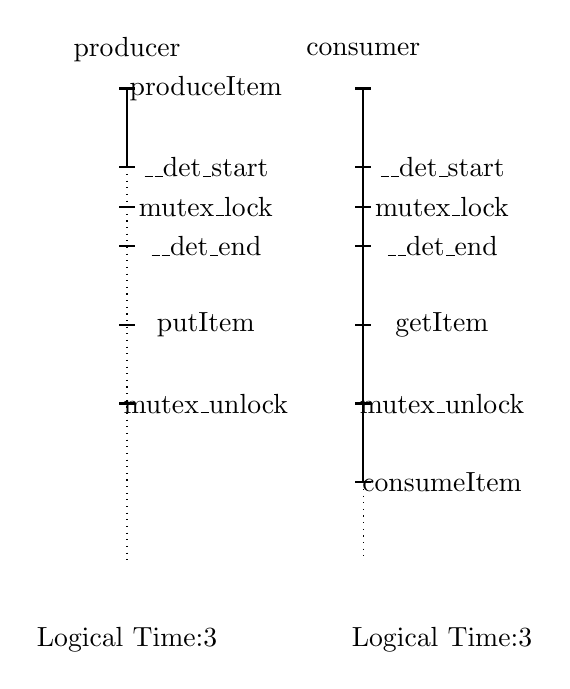
\begin{tikzpicture}
   \draw[thick] (0,4) --  (0,5); 
   \draw[dotted] (0,4) --  (0,-1);
   
   \node[align=right] at (0,5.5) {producer};
   \node[align=right] at (1,5) {produceItem};
   \draw[thick] (-0.1,5) -- (0.1,5);
   \node[align=right] at (1,4) {\_\_det\_start};
   \draw[thick] (-0.1,4) -- (0.1,4);
   \node[align=right] at (1,3.5) {mutex\_lock};
   \draw[thick] (-0.1,3.5) -- (0.1,3.5);
   \node[align=right] at (1,3) {\_\_det\_end};
   \draw[thick] (-0.1,3) -- (0.1,3);
   \node[align=right] at (1,2) {putItem};
   \draw[thick] (-0.1,2) -- (0.1,2);
   \node[align=right] at (1,1) {mutex\_unlock};
   \draw[thick] (-0.1,1) -- (0.1,1);   
   \node[align=right] at (0,-2) {Logical Time:3};
   
   \draw[thick] (3,0) --  (3,5); 
   \draw[dotted] (3,0) --  (3,-1);
   
   \node[align=right] at (3,5.5) {consumer};
   \node[align=right] at (4,5) {};
   \draw[thick] (2.9,5) -- (3.1,5);
   \node[align=right] at (4,4) {\_\_det\_start};
   \draw[thick] (2.9,4) -- (3.1,4);
   \node[align=right] at (4,3.5) {mutex\_lock};
   \draw[thick] (2.9,3.5) -- (3.1,3.5);
   \node[align=right] at (4,3) {\_\_det\_end};
   \draw[thick] (2.9,3) -- (3.1,3);
   \node[align=right] at (4,2) {getItem};
   \draw[thick] (2.9,2) -- (3.1,2);
   \node[align=right] at (4,1) {mutex\_unlock};
   \draw[thick] (2.9,1) -- (3.1,1);
   \node[align=right] at (4,0) {consumeItem};
   \draw[thick] (2.9,0) -- (3.1,0);
   \node[align=right] at (4,-2) {Logical Time:3};   
\end{tikzpicture}
\caption{An example of logical time imbalance.}
\label{fig:p2-1}
\end{figure}

In Figure~\ref{fig:p2-1}, we show a particular execution point of the producer-consumer model that corresponds to the program shown in Figure~\ref{fig:p1-1}. In this case, consumer reaches consumeItem with logical time 3 and has the token. Assume the real execution time of consumeItem is 10s, which means that when the consumer reaches \_\_det\_end, it would be at least 10s later, that is, the producer has to wait at \_\_det\_start for at least 10s. However we've already enforces the access order of the mutex, the execution out of the critical section should go in parallel since threads don't communicate at that part, this waiting time is totally unnecessary. In a more complex application with more synchronization, this kind of waiting will break a parallel program into a serial program.

Logical time imbalance can happen in two cases:
\begin{itemize}
  \item A task is running in the userspace for a long time.
  \item A task is sleeping in the kernel space for a long time.
\end{itemize}

In the upcoming sections we will discuss the solution of each of the cases.
\subsection{Execution Time Profiling}
\subsection{Non-deterministic External Events}
\begin{figure*}[ht]
\centering
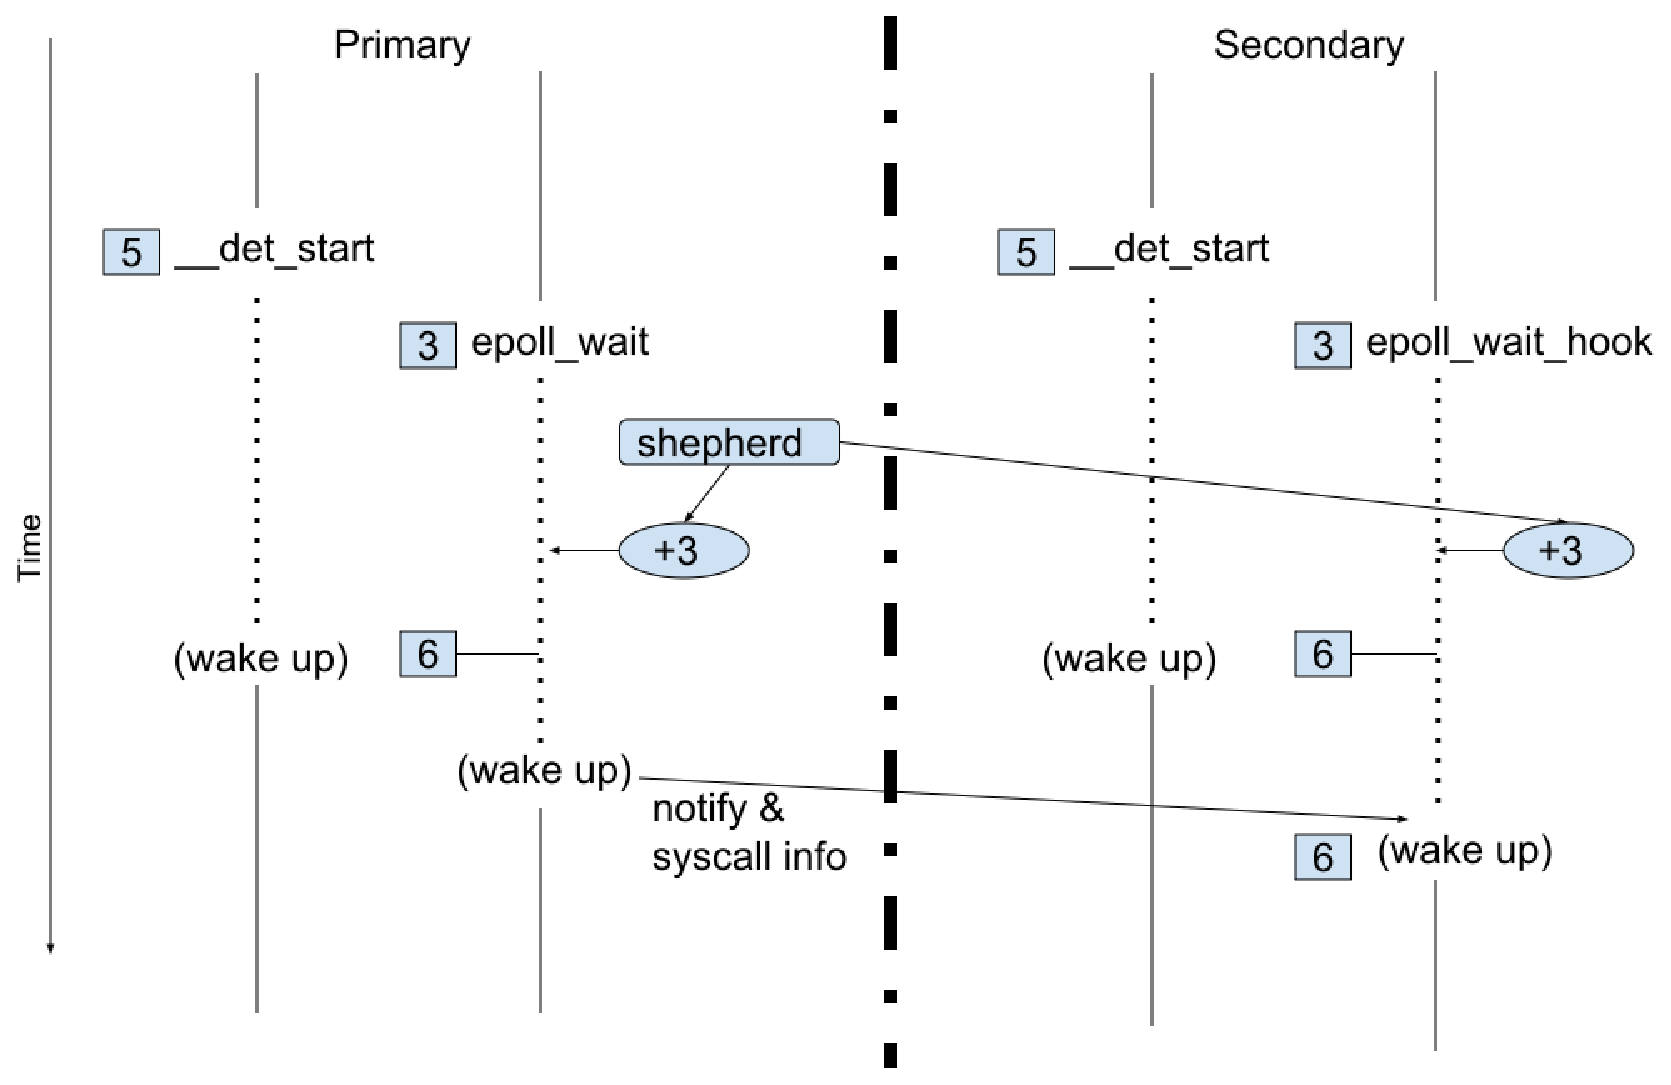
\includegraphics[width=1.5\columnwidth]{figures/tickbump}
\caption{ In this example, tick shepherd detects the token is on a thread sleeping in epoll\_wait, so it bumps its tick by 3 and sends this info to the secondary so that the token can leave this thread. And after the primary returns from epoll\_wait, it sends a message along with the epoll\_wait\'s output to the secondary, so that the corresponding thread can start to execute its epoll\_wait and uses the output from the primary as its own output. }
\label{f:tick_bump}
\end{figure*}

Some blocking system calls would put the caller into sleep. When a thread holding a token reaches such a system call, the token might be on this thread for a long time. Especially for system calls like epoll\_wait, poll and accept, the arrival time of the event is non-deterministic, as a result, we cannot simply use \dettick\ to increase the logical time with a predefined value. In order to let the token passing keep going with those blocking system calls, a "Tick Shepherd" is implemented to dynamically bump the logical time of the threads that are sleeping on external events. The Shepherd is a kernel thread which is mostly sleeping in the background, whenever the token is passed on to a thread that is sleeping on external events or a thread is going to sleep with the token, the shepherd will be woken up to increase its logical time and send the delta to the replica. In the meanwhile the corresponding system call on the replica will be blocked at the beginning, and bump its logical time according to the information from the primary. The syscall on the secondary doesn't proceed until the primary returns from the syscall. In this way we can make sure that when both of the syscalls wake up from sleeping, all the replicas will end up with a consistent state, in terms of logical time.
